
Każda zakładka z obrazem lub obrazami jest implementowana przez klasę \sokarclass{DicomView}.

Interfejs graficzny \sokarclass{DicomView} posiada następujące elementy:
\begin{itemize}
    \item pasek narzędzi znajdujący się na górze - implementowany za pomocą klasy \sokarclass{DicomToolBar}, opisany w sekcji \ref{sec:sokar-dicomtoolbar}
    \item miejsce na scene z obrazem DICOM na środku - implementowany za pomocą klasy \sokarclass{DicomGraphics}, opisany w sekcji \ref{sec:sokar-dicomgraphics}
    \item suwak filmu w dolnej części - implementowany za pomocą klasy \sokarclass{MovieBar}, opisany w sekcji \ref{sec:sokar-moviebar}
    \item podgląd miniaturek obrazów w prawej części - implementowany za pomocą klasy \sokarclass{FrameChooser}, opisany w sekcji \ref{sec:sokar-framechooser}
\end{itemize}

Dodatkowo posiada obiekt \sokarclass{DicomSceneSet}, który jest zbiorem obrazów opisany w sekcji \ref{sec:sokar-scenesets}.
\sokarclass{DicomView} łączy zdarzenia wysyłane przez wszystkie obiekty.

Poniżej jest opisane zachowanie tych elementów:

\subsection{Elementy interfejsu graficznego}

\begin{figure}[!htbp]
    \centering
    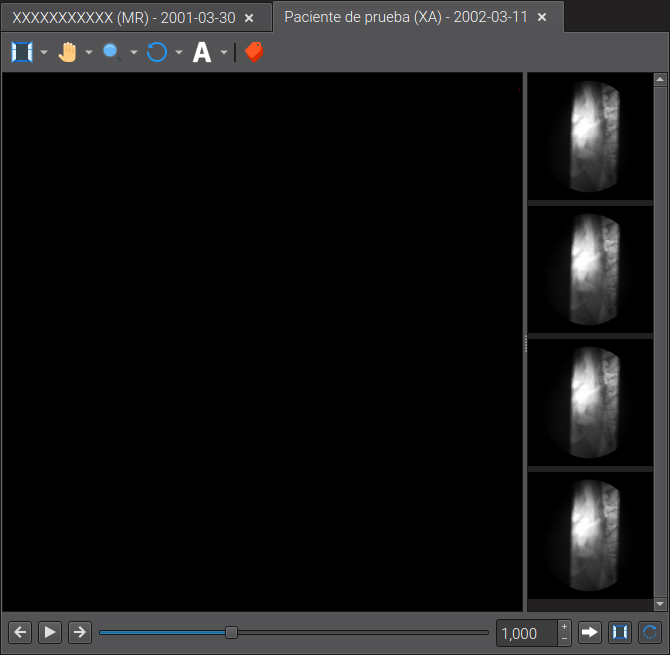
\includegraphics[width=\textwidth]{img/sokar-dicomview-001.png}
    \caption{Wygląd DicomView wraz z numeracją elementów interfejsu. Zdjęcie własne.}
    \label{fig:sokar-dicomview001}
\end{figure}

\subsubsection{\sokarclass{DicomToolBar}}
\label{sec:sokar-dicomtoolbar}
\label{sec:sokar-dicomtoolbar}
\par
Pasek narzędzi znajdujący się na górze, implementowany przez klasę \sokarclass{DicomToolBar}, dziedziczącą po klasy \qtclass{QToolBar}.
Posiada on zespół ikonek z rozwijalnymi menu kontekstowymi.

\par
Kliknięcie odpowiedniej ikony spowoduje wysłanie sygnału do obecnie wyświetlanej sceny.
Są dwa sygnały możliwe do wysłania \sokarfunction{DicomToolBar}{stateToggleSignal} lub \sokarfunction{DicomToolBar}{actionTriggerSignal}.
Pierwszy sygnał oznacza zmianę stanu paska, czyli sposób obsługi myszki, zawierał jeden argument: stan (typu \cppcode{enum}).
Sygnał ten okazał się bez użyteczny i nie jest wykorzystywany przez scene.
Drugi oznacza akcje, sygnał akcji, która powinna być wykonana na przez scenę, zawiera dwa argumenty: typ akcji (typu \cppcode{enum}) i stan akcji (typu \cppcode{bool} z domyślną wartością \cppcode{false}).

Ikony na pasku:
\begin{itemize}
    \item Okienkowanie (1)

          Stan: \cppcode{Windowing}.
          Oznacza, że horyzontalny ruch myszki powinien zmieniać szerokość okna, a wertykalny środek okna.
          Przycisk jest aktywny tylko wtedy gdy na obecna scena posiada obraz monochromatyczny.

    \item Przesuwanie (2)

          Stan: \cppcode{Pan}.
          Oznacza, że ruch myszki powinien przesuwać obraz na scenie w prawo, lewo, góra, dół, kiedy jest wciśnięty klawisz myszy.

          Rozwijalne menu zawiera tylko jedne element \enquote{Move To Center} wysyłający sygnał akcji z argumentem \cppcode{ClearPan}.

    \item Skalowanie (3)

          Stan: \cppcode{Zoom}.
          Oznacza, że ruch myszki powinien skalować obraz kiedy jest wciśnięty klawisz myszy.

          Menu rozwijalne:
          \begin{itemize}
              \item Fit To Screen --- Dopasuj do ekranu

                    Akcja: \cppcode{Fit2Screen}.

                    Po otrzymaniu sygnału obraz na scenie powinien dopasować swoją wielkość do wielkości sceny

              \item Original Resolution --- Skala jeden do jednego

                    Akcja: \cppcode{OriginalResolution}.

                    Po otrzymaniu sygnału obraz na scenie powinien dopasować swoją wielkość jeden do jedne w stosunku do piksela na ekranie.

          \end{itemize}

    \item Rotacja (4)

          Stan: \cppcode{Rotate}.
          Oznacza, że ruch myszki powinien obracać obrazem znajdującym się na scenie.

          Menu rozwijalne:
          \begin{itemize}
              \item Rotate Right --- Obróć w prawo

                    Akcja: \cppcode{RotateRight90}.

                    Po otrzymaniu sygnału obraz na scenie powinien obróć się o 90 stopni w prawo.

              \item Rotate Left --- Obróć w lewo

                    Akcja: \cppcode{RotateLeft90}.

                    Po otrzymaniu sygnału obraz na scenie powinien obróć się o 90 stopni w lewo.

              \item Flip Horizontal --- Odbij lustrzanie poziomo

                    Akcja: \cppcode{FlipHorizontal}.

                    Po otrzymaniu sygnału obraz na scenie powinien odbić się lustrzanie poziomo.

              \item Flip Vertical --- Odbij lustrzanie pionowo

                    Akcja: \cppcode{FlipVertical}.

                    Po otrzymaniu sygnału obraz na scenie powinien odbić się lustrzanie pionowo.

              \item Clear Transformation --- Wyczyść przekształcenia obrotu

                    Akcja: \cppcode{ClearRotate}.

                    Po otrzymaniu sygnału obraz na scenie powinien wyczyścić transformatę obrotu.

          \end{itemize}
    \item Informacje na obrazie (5)

          Ten element potrafi wyłączyć wyświetlanie niektórych elementów na scenie.
          Kliknięcie go odznacza lub zaznacza wszystkie pozycje w menu kontekstowym.
          Wszystkie pozycje są pozycjami odznaczanymi.

          Menu rozwijalne:
          \begin{itemize}
              \item Patient Data --- Dane pacjenta

                    Akcja: \cppcode{PatientData}.

                    Po otrzymaniu sygnału obiekt klasy \sokarclass{PatientDataIndicator} znajdujący się na scenie powinien pokazać lub ukryć się w zależności od stanu pozycji.

              \item Hospital Data --- Dane szpitala

                    Akcja: \cppcode{HospitalData}.

                    Po otrzymaniu sygnału obiekt klasy \sokarclass{HospitalDataIndicator} znajdujący się na scenie powinien pokazać lub ukryć się w zależności od stanu pozycji.
              \item Image Acquisition --- Dane akwizycji

                    Akcja: \cppcode{ModalityData}.

                    Po otrzymaniu sygnału obiekt klasy \sokarclass{ModalityIndicator} znajdujący się na scenie powinien pokazać lub ukryć się w zależności od stanu pozycji.

          \end{itemize}

    \item Tagi (5)

          Akcja: \cppcode{OpenDataSet}.

          Kliknięcie tego przycisku wyśle prośbę o otworzenie okna ze zbiorem elementów danych pliku obrazu, który jest obecnie wyświetlany na scenie.

\end{itemize}

\subsubsection{\sokarclass{DicomGraphics}}
\label{sec:sokar-dicomgraphics}

\subsubsection{\sokarclass{MovieBar}}
\label{sec:sokar-moviebar}

\par
Jest paskiem filmu w dolnej części \sokarclass{DicomView}.
Element graficzny ma dostęp do sekwencji scen i ukrywa swoją obecność przed użytkownikiem, kiedy w sekwencji jest tylko jedna scena.

\par
Pasek jest podzielony na trzy części: trzy przyciski znajdujące się po lewej, pasek pokazujący postępu sekwencji na środku i prządka z trzema przyciskami po prawej.

\par
Trzy lewe przyciski odpowiadają za poruszanie się po sekwencji.
Wciśniecie pierwszego przycisku (z indeksem 8 na rysunku \ref{fig:sokar-dicomview001}) powoduje zatrzymanie upływu sekwencji i wysłanie sygnału \sokarfunction{SceneSequence}{stepBackward} do sekwencji.
Wciśniecie drugiego przycisku (9) powoduje włączenie lub wyłączenie upływu sekwencji.
Wciśniecie trzeciego przycisku (10) powoduje zatrzymanie upływu sekwencji i wysłanie sygnału \sokarfunction{SceneSequence}{stepForward} do sekwencji.
\par
Pasek (11) pokazujący postępu sekwencji jest obiektem klasy \qtclass{QSlider}.
Odświeżanie paska jest wrażliwe na sygnał \sokarfunction{SceneSequence}{steped} of sekwencji.
\par
Elementy po prawej stronie definiuje parametry trybu filmowego.
Prządka (12), element do wprowadzania liczby zmiennoprzecinkowej klasy \qtclass{QDoubleSpinBox}.
Im większa wartość liczby tym klatki filmu są dłużej wyświetlane.
Drugi (13) przycisk pozwala zmienić sposób przemiatania.
Trzeci (14) przycisk wymusza tryb jednego okna dla wszystkich klatek filmu.
Jeżeli mamy załadowanych wile obrazów tego samego badania, to nie koniecznie muszą mieć to samo okno.
Dodatkowo ten tryb pozwala wprowadzić jednolite okienko dla wszystkich klatek po zmianie parametrów tego okienka na jednej klatce.
Czwarty (15) i ostatni przycisk służy do użycia jednej macierzy transformaty na wszystkich klatkach.

\paragraph*{Tryb filmowy}

\par
Tryb filmowy można aktywować jedynie wtedy gdy w sekwencji scen jest więcej niż jedna scena.
Włączenie trybu filmowego polega na stworzeniu obiektu klasy \sokarclass{MovieMode}.
Obiekt ten zapisuje wskaźnik go obecnie wyświetlanej sceny, to czy powinno być użyte to samo okno, oraz to czy powinna być używana ta sama transformata.
Następnie obiekt ten jest wysyłany do wszystkich scen w sekwencji.
Uruchamiany jest timer, obiekt klasy \qtclass{QTimer}, na czas równy czasu trwania sceny zapisanego w kroku przemnożonego przez liczbę z prządki.
Po upływie timera, wstawiana jest nowa scena za pomocą sygnały \sokarfunction{MovieBar}{setStep}, a timer jest ustawiany nan nowo.

\subsubsection{\sokarclass{FrameChooser}}
\label{sec:sokar-framechooser}

Ten element to wybór scen za pomocą ikon, implementowany przez klasę \sokarclass{DicomView}.
Element, podobnie jak pasek filmu ma dostęp do sekwencji scen i ukrywa swoją obecność przed użytkownikiem, kiedy w sekwencji jest tylko jedna scena.
Po wciśnięciu ikony jest zmieniana scena.